\documentclass[11pt]{standalone}
\usepackage{color}
\usepackage[cmyk]{xcolor}
\usepackage{amsmath}
\usepackage{xltxtra}
\usepackage{libertine}

\usepackage{tikz}
\usetikzlibrary{intersections,arrows,calc}
% \tikzstyle{every picture}+=[thick]

\usepackage[active,tightpage]{preview}
\PreviewEnvironment{tikzpicture}
\setlength\PreviewBorder{1pt}%

\newcommand{\qbar}[1][b]{\kern 0.06em \overline{\kern -0.06em \text{#1} \kern -0.04em} \kern 0.04em}
\newcommand{\Bs}{\text{B}_\text{s}^\text{0}}
\newcommand{\kaon}[1][0]{\text{K}^\text{#1}}
\newcommand{\Kp}{\kaon[+]}
\newcommand{\Km}{\kaon[--]}
\newcommand{\pimes}[1][]{\text{π}^\text{#1}}
\newcommand{\lmu}[1][]{\text{μ}^\text{#1}}

\begin{document}
\sffamily
\begin{tikzpicture}
  \node[anchor=south]{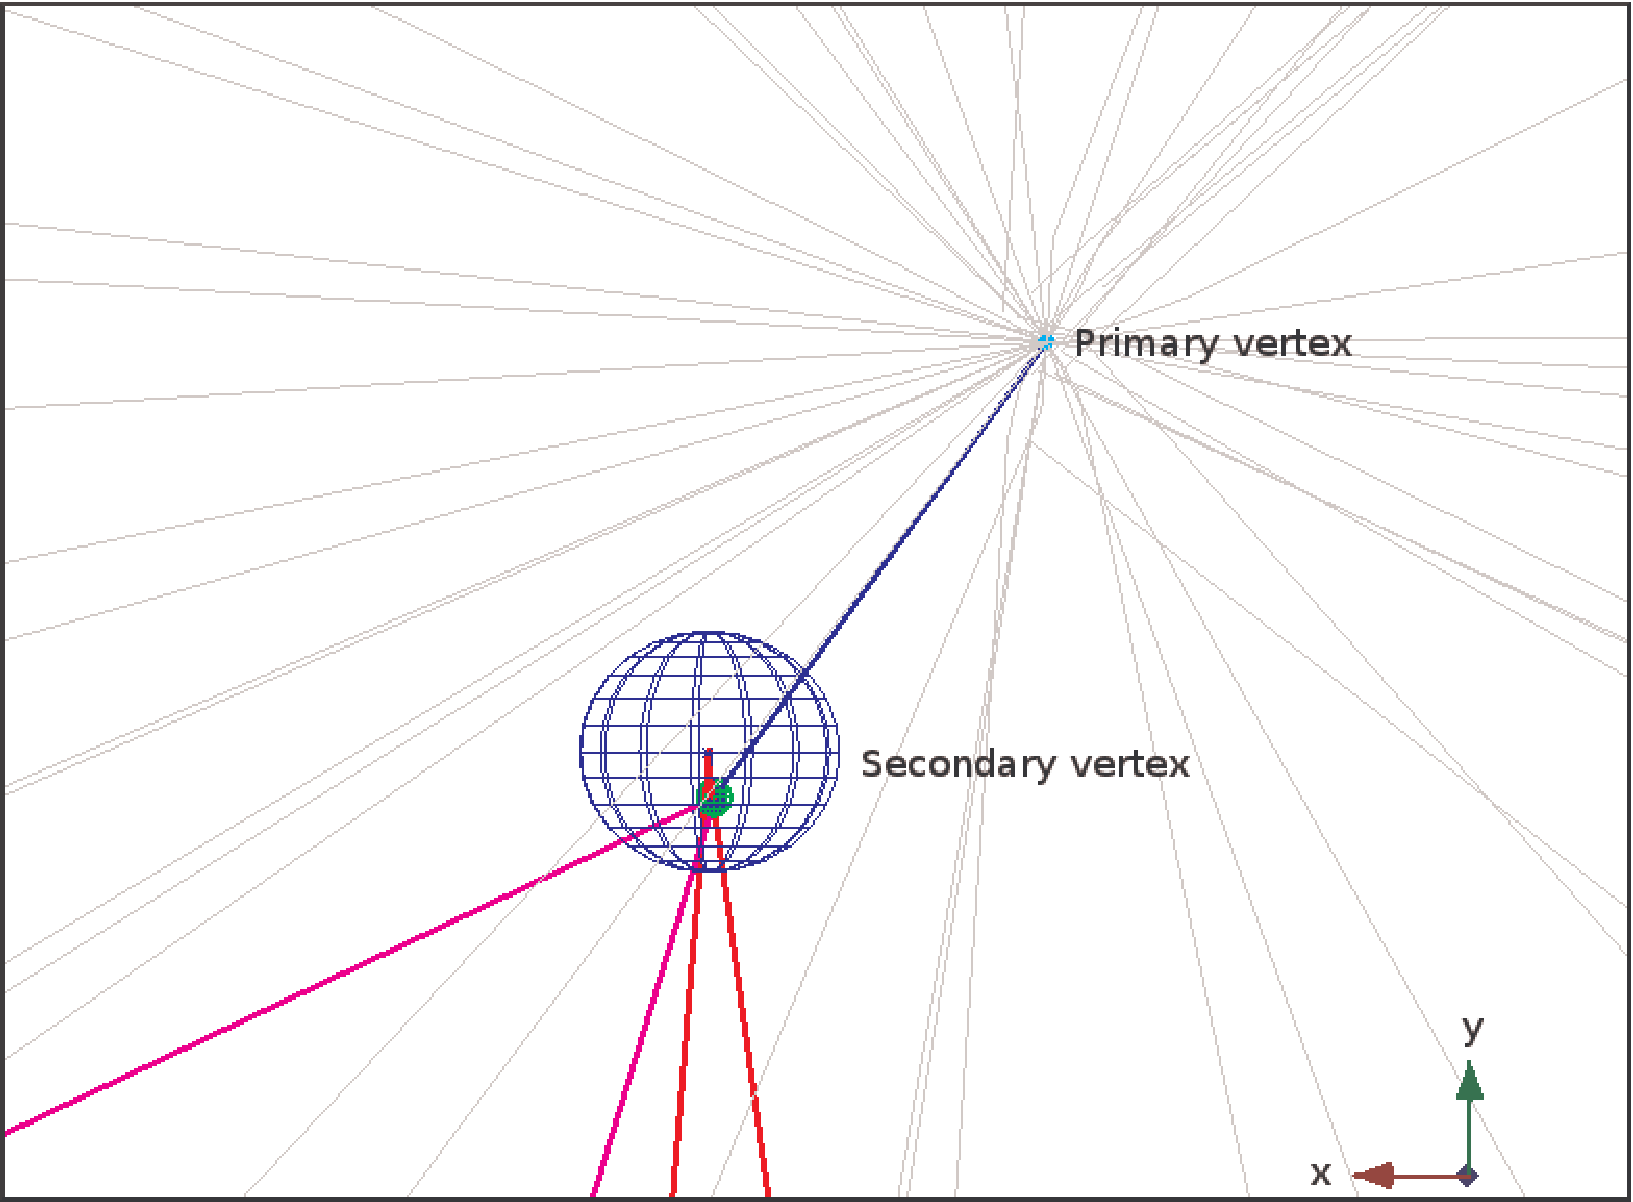
\includegraphics[width=0.98\textwidth]{../vertices_CMYK}};
  \node at (  0.65, 4.5 )  {$\Bs$};
  \node at ( -0.14, 1.1 )  {$\Kp$};
  \node at ( -0.77, 0.45 ) {$\Km$};
  \node at ( -3.5,  1.54 ) {$\lmu[+]$};
  \node at ( -1.86, 0.6 )  {$\lmu[--]$};
\end{tikzpicture}
\end{document}
